\thispagestyle{fancy}
\begin{center}
	\LARGE{\textbf{Teorema de Thevenin}}
\end{center}
\section{Objetivos}
Al finalizar esta experiencia, usted estará capacitado para:
\begin{enumerate}
	\item Determinar \textbf{V (Thevenin)} a partir de mediciones realizadas con un voltímetro.
	\item Determinar \textbf{R (Thevenin)} a partir de mediciones realizadas con un Óhmimetro. 
	\item Conectar el circuito equivalente de Thevenin.
	\item Probar el circuito original y circuito equivalente de Thevenin para comprobar si proveen la misma corriente y tensión con diferentes cargas.
\end{enumerate}
\section{Conocimientos previos}
El teorema de Thevenin puede ser usado para convertir cualquier red de dos terminales en un circuito equivalente que contiene una fuente de tensión en serie con una resistencia; el equivalente Thevenin.
Para realizar la conversión, calcule en primer término la salida en circuito abierto. Este será el valor de la tensión equivalente de Thevenin o V (Thevenin).
Luego, cortocircuite todas las fuentes de tensión sin cargar la salida (sin conectar). Calcule la resistencia equivalente se ve desde los terminales de salida. Este es el valor de la resistencia R (Thevenin).
\section{Autoevaluación de entrada}
\begin{enumerate}
	\item La tensión de Thevenin de define como: la tensión entres dos terminales (A y B)
	\\ Antes de comenzar esta sección, usted debe saber:
	\begin{enumerate}
		\renewcommand{\theenumi}{\alph{enumi}}
		\item Cómo hallar V (Thevenin) en un circuito eléctrico.
		\item Cómo hallar R (Thevenin) en un circuito eléctrico.
		\item Convertir cualquier circuito eléctrico en su equivalente Thevenin.
	\end{enumerate}
	\item La resistencia de Thevenin es medida: agregando la fuente de voltaje y la corriente, también se puede cortocircuitar si es una fuente de tensión o abriendo si es una fuente de corriente
\end{enumerate}
\section{Equipo}
Para realizar la experiencia de laboratorio, se precisa el siguiente equipo:
\begin{enumerate}
	\item Modulo de experimentos.
	\item Miliamperímetro.
\end{enumerate}
\section{Procedimiento}
\begin{enumerate}
	\item Estudie y efectué los cálculos para el circuito de la figura 1 de la izquierda (el circuito original):
	\\
	\begin{figure}[h]
		\centering
		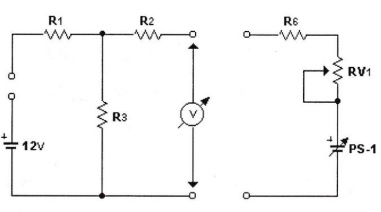
\includegraphics[scale=1]{imagenes/4.1}
		\caption{Circuito original}
	\end{figure}
	\item Conecte en el circuito que se muestra en la figura 1.
	\item Mida la tensión de salida en circuito abierto de la red. Anote el resultado. Este es el valor de V (Thevenin).
	\\ V (Thevenin)
	\item Lleve la salida de la fuente PS-1 del circuito de la derecha (Circuito equivalente Thevenin) a la tensión de salida de Thevenin de 6v.
	\begin{figure}[h]
		\centering
		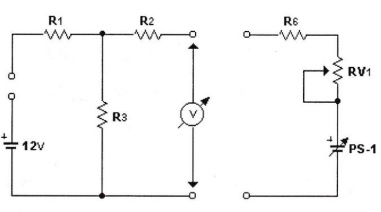
\includegraphics[scale=1]{imagenes/4.1}
		\caption{Segundo circuito}
	\end{figure}
	\item Midamos nuevamente el circuito de la figura 1 (lado izquierdo).
	\item Para medir R(Thevenin), debe colocarse un \textbf{cortocircuito} en vez de la fuente de 12v.
	\begin{enumerate}
		\item Desconecte los terminales de la fuente, y ponga el terminal izquierdo de $R_{1}$ a masa.
		\item Conecte el multímetro como Ohmímetro en los terminales de salida.
		\item Mida la resistencia de salida y anótela. Esta es R (Thevenin).
		\\ R (Thevenin) = 4.9$\Omega$
	\end{enumerate}
	\item Retire el cortocircuito de los terminales de la fuente de 12v.
	\item Conecte el multímetro como ohmimetro en $R_{1}$ y $R_{6}$ y luego ajuste $RV_{1}$ hasta que los valores de la resistencia sean iguales a R (Thevenin) = $0,61k\Omega$.\\
Usted ha comparado que la fuente de alimentación PS-1 y $RV_{1} + R_{6}$ forman el equivalente Thevenin del circuito formado por una fuente de alimentación de $12v$, $R_{1}, R_{2}$ y $R_{3}$.
\\
Para verificar que el circuito original y su equivalente Thevenin son realmente equivalentes, realicemos algunas mediciones.
\begin{table}[h]
	\centering
	\begin{tabular}{|c|c|c|}
		\hline
		\textbf{Carga}&\textbf{$V_{sal} (V)$}&\text{$I_{sal} (mA)$}\\
		\hline
		$R_{4} =1.5k$&0.459V&0.30mA\\
		\hline
		$R_{5}=1.8k$&0.529V&0.289mA\\
		\hline
		Cortocircuito&1.8V&0.42mA\\
		\hline
	\end{tabular}
	\caption{Circuito original}
\end{table}
\\
Cargue el circuito original con $R_{4}$. Mida $V_{sal}$ y $I_{sal}$ e registre en el cuadro 1.
\\
Reemplace la carga $R_{4}$ con $R_{5}$. Mida $V_{sal}$ y  $I_{sal}$ e registre en el el cuadro 1.
\\
Reemplace $R_{5}$ con un cortocircuito. Mida $V_{sal}$ y $I_{sal}$ e registre en el cuadro 1.
\item Repita estas pruebas en el circuito equivalente de Thevenin; cargue al circuito original con $R_{4}$. Luego, utilizamos $R_{5}$ como carga, repita el procedimiento. Finalmente, cortocircuite la salida.
\\ 
Para cada valor de la carga, mida $V_{sal}$ y $I_{sal}$ y registre en el cuadro 2.
\begin{table}[h]
	\centering
	\begin{tabular}{|c|c|c|}
		\hline
		\textbf{Carga}&\textbf{$V_{sal} (V)$}&\text{$I_{sal} (mA)$}\\
		\hline
		$R_{4}=1.5k$&0.461V&0.31mA\\
		\hline
		$R_{5}=1.8k$&0.531V&0.292mA\\
		\hline
		Cortocircuito&1.8V&0423mA\\
		\hline
	\end{tabular}
	\caption{Circuito circuito equivalente de Thevenin}
\end{table}
	\item En esta parte del experimento, altere el circuito con otros valores para los resistores.
	\\ Aplique sus conocimientos teóricos para determinar qué parte del circuito ha cambiado.
	$R_{7}= 4.7k, R_{8}=1.5k, R_{9}=2.7k$
	\item Para el circuito que ha modificado. Repita el procedimiento para medir v (Thevenin) y R (Thevenin).
	\item Mida la tensión de salida a circuito abierto. Este valor de V(Thevenin), ingréselo:
	\\ V (Thevenin) = 4.38V
	\item Para R (Thevenin), cortocircuite la entrada al circuito reemplazando a la fuente de 12v.
	\begin{enumerate}
		\item Desconecte los terminales de la fuente, y ponga el terminal izquierdo de $R_{1}$ a masa.
		\item Conecte el multímetro como ohmímetro en los terminales de salida.
		\item Mida la resistencia de salida anótela. Esta es R (Thevenin).
		\\ R (Thevenin) = 3.215$\Omega$
	\end{enumerate}
	\item ¿Qué resistor fue desconectado?
	\\ se desconecto la resistencia $R_{3}$
	\item En este segundo ejercicio de experiencia, un resistor ha sido cortocircuito. Repita el procedimiento para volver a medir R (Thevenin) y V (Thevenin).
	\item Mida la tensión de salida en circuito abierto de la red. Este es el valor de V (Thevenin). 
	\\ V (Thevenin) = 12V 
	\item Para medir R (Thevenin), cortocircuite la entrada al circuito (que la fuente de alimentación de $12V$).
	\\ Conecte el multímetro en los terminales de salida del circuito, mida y registre la resistencia de salida. Esta es R (Thevenin).
	\\ R (Thevenin)= 1.1$k\Omega$
	\item El componente cortocircuito es la fuente de tensión
\end{enumerate}
\section{Autoevaluación}
\begin{enumerate}
	\item La tensión de Thevenin es mediada en los terminales (A y B)
	\item Cuando una tensión inicial $6v$ se conecta en serie con tres resistores iguales de $2.3\Omega$, el circuito equivalente de Thevenin es
	\item Evalué el circuito siguiente
	\begin{figure}[h]
		\centering 
		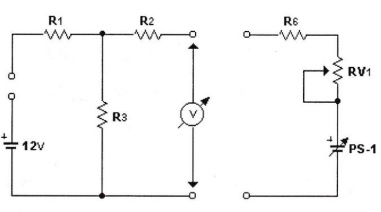
\includegraphics[scale=1]{imagenes/4.1}
		\caption{Circuito a evaluar}
	\end{figure}
	\begin{enumerate}
		\item Desconecte $R_{3}$ produce un lazo son resistencia en serie 
		\item Cortocircuitar $R_{3}$ produce dos lazos con resistencias en paralelo
	\end{enumerate}
\end{enumerate}
\section{Conclusión}
En este laboratorio, la teoría de Thevenin es muy común para realizar las transformaciones de circuitos de una manera mas sencillas, todo ello se puede hacer por nodos o mallas de acuerdo al circuito que se deba convertir.
